\documentclass[
  10pt,
  a4paper,
  oneside,
  headers,
  headinclude,
  footinclude,
  BCOR5mm,
]{article}
\usepackage{float}
\usepackage{ragged2e}
\usepackage{graphicx}
\usepackage{subcaption}
\usepackage{beramono}
\usepackage[utf8]{inputenc}
\usepackage{listings}
\usepackage{wrapfig}

\graphicspath{ {./images/} }
\renewcommand{\figurename}{Abb.}

\title{IT Projekt}
\date{06.05.2019}
\author{Ivaylo Lenkov Ivanov}

\begin{document}

\begin{titlepage}
  \maketitle
  \tableofcontents
  \pagebreak
  \listoffigures
\end{titlepage}

\section{Einführung}
Für ein Hauptziel hat dieses Projekt eine virtuelle Umgebung zu bilden und in
dieser Umwelt die grundlegende Physik zu simulieren. Die virtuelle Welt ähnelt
ein Computerspiel. \\
Der Benutzer steuert eine virtuelle Figur, die Avatar genannt ist.
Der Avatar kann sich in dem Terrain bewegen und Eiszapfen in jeder Richtung
feuern. Die Anfangsszene des Spiels hat vier Spielobjekte --- drei Kasten und
ein Stein. \\
Mit den Kisten kann der Anwender interagieren. Das heißt, dass der Benutzer sie
leiten kann und auch auf sie Eiszapfen zu schießen. Das kann zu der
Zerstörung diesen Kästen führen. Der Stein, der auch statisch Spielobjekt
genannt wird, funktioniert wie eine Wand. Er ist unbeweglich und auch
unverwüstlich. \\
In meisten virtuellen Produkten wird die Information durch irgendeiner Art von
Animation vorgestellt. Unter Animation versteht man sichtbare Bewegung. Das kann
sehr wichtig sein, weil es ein Software viel mehr intuitiv macht. In den meisten
Fällen die Systeme, die solche Lebhaftigkeit machen, sind Physik-Engines. \\
Implementieren die Physik in einem virtuellen Welt macht die Animationen, die
Bewegungen und die Wechselwirkungen in diesem Welt immer flüssiger und
realistischer und gibt immersives Erlebnis. Die Bilder sieht schöner und
lebendiger aus. Diese Eigenschaften sind wichtig nicht nur in den
Computerspielen, sonder auch in der virtuelle Realität, in der Software für
visuelle Effekte und in den Anwendungen für Physik Simulation und für
Animation. \\
Für dieses Projekt wird ein Spiel erstellt, wo die grundlegende physikalischer
Gesetze gelten. In der virtuellen Welt gibt es eine Implementation von
Beschleunigung, Kollisionserkennung, Kollisionsauflösung und elementare
Teilchen. \\
Solche Umfeldern sind kompliziert und brauchen viel Speicher. Man soll auch auf
der Leistung der Software passen. Diese virtuelle Umgebung wird durch die
Programmiersprache C++ erstellt. Auf diese Weise wird der Speicher sehr streng
kontrolliert. Die Sprache erlaubt bessere Performance und macht die Anwendung
auch portabel. Für den Computergrafik Teil wird die Programmiere-Bibliothek
``SDL2'' benutzt. Die ``png'' Bilder werden mit der Hilfe von der
Programmiere-Bibliothek ``SDL2-image'' geladen. \\

\section{Überblick --- Bestandteile und Funktionsweise}
Wenn man das ganze Projekt betrachtet, kann man die folgende Teile des Spiels
bemerken --- Initialisierung, die Spiel-Schleife und Befreiung des Speichers. \\
Während der Initialisierung wird das Fenster, wo die virtuelle Welt dargestellt
wird. Die Texturen werden geladen. Danach wird die initiale Szene des Spiels
geschaffen.

\begin{figure}[h]
  \centering
  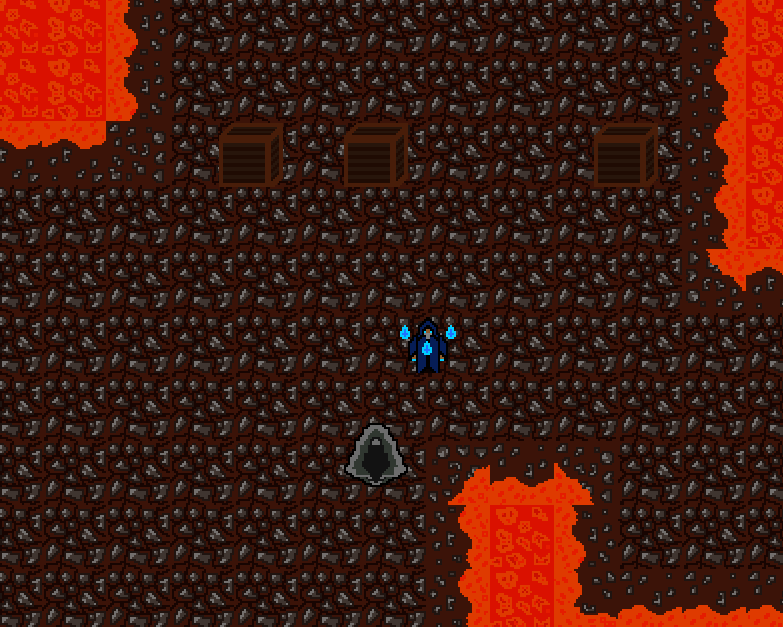
\includegraphics[scale=0.25]{VirtualEnvironment}
  \caption{Die initiale Szene des Spiels}
  \label{fig:Umgebung}
\end{figure}

Die nächste Phase ist die Spiel-Schleife. Das ist der Kern jedes Spiels --- ein
endlose, aber überwachte Kreislauf. Hier werden die Dynamik und die
Interaktivität der virtuellen Welt durchgeführt. Die folgende 4 teile werden
erkennt --- das Normieren von der Bildrate, eine Prüfung auf Ausfahrt,
Aktualisieren der Spielszene und Vorbereiten den Objekten zum Rendern und das
Rendern der Änderungen. Damit die Bildfrequenz normieren können, wird die Zeit
der Rahmen für ein Iteration der Spiel-Schleife gefunden. Wenn diese Uhrzeit
kleiner als die festgelegte ist, dann wird die Bildrate nachdrücklich verzögert.
Das ist wichtig, weil auf diese Weise die verschiedene Computer die gleiche
Bildfrequenz haben werden. \\
Der Kreis ist endlos, aber das bedeutet nicht, dass das Spiel kein Schluss hat.
Drücken einer Taster wird als ein Event registriert. Auf diese Weise
kommuniziert der Benutzer mit der virtuellen Umgebung. Solche Veranstaltungen
werden gesammelt und werden bearbeitet. In diesem Projekt bricht die Schleife
das Drücken auf den Knopf ``ESC''. \\
Die Update-Phase des Spiel-Loops wird zunächst sichergestellt, dass alle
Objekte, die in der Szene zerstört oder nicht mehr benötigt werden, keinen
Speicher mehr brauchen. Mit anderen Worten, hält die Liste der Objekte, die
verfolgt werden, aktuell. Dies ist entscheidend für die Leistung des Spiels.
Nachdem es bestätigt wurde, welche Spielobjekte in der Spielszene aktiv sind,
werden ihre Position und ihr Zustand aktualisiert. \\
Danach wird festgestellt, ob ein Spielobjekt mit einem anderen kollidiert.

\begin{figure}[h]
  \begin{subfigure}{0.3\textwidth}
    
\includegraphics[width=0.5\linewidth, height=1.9cm]{Box}
    \caption{Kasten}
    \label{fig:Kasten}
  \end{subfigure}
  \begin{subfigure}{0.3\textwidth}
    
\includegraphics[width=0.5\linewidth, height=1.9cm]{Stone}
    \caption{Stein}
    \label{fig:Stein}
  \end{subfigure}
  \begin{subfigure}{0.3\textwidth}
    
\includegraphics[width=0.5\linewidth, height=1.9cm]{frostbolt}
    \caption{Projektil}
    \label{fig:Projektil}
  \end{subfigure}

  \caption{Spielobjekte}
  \label{fig:Spielobjekte}
\end{figure}

Auf der Grundlage ihrem Typ wird eine bestimmte Art von Kollisionsauflösung
ausgegeben. Die Auflösungen sind unterschiedlich, daher müssen sie getrennt
werden.

\newpage %% New page because of formatting issues
\begin{wrapfigure}{l}{0.3\textwidth}
    \centering
    \includegraphics[width=0.25\textwidth, height=3cm]{MageCHaracter}
    \caption{Avatar}
    \label{fig:Avatar}
\end{wrapfigure}

In diesem Projekt wird bei der ersten Kollision geprüft, ob der Avatar des
Spielers mit einem anderen starren Körper kollidiert ist. Wenn dieser Schritt
bestanden ist, kommt der Test, dass das Projektil mit einem beliebigen Objekt in
der Spielszene kollidiert. Zunächst wird festgestellt, ob ein anderer Avatar
getroffen wurde, was im aktuellen Projektstatus überflüssig ist, da der Benutzer
der einzige ist, der einen hat. Wenn dann ein Projektil ein Spielobjekt
geschlagen hat, werden zwei Arten von Lösungen implementiert. Wenn das
getroffene Spielobjekt statisch ist, wird das Projektil einfach zerstört. Wenn
das Spielobjekt jedoch beweglich ist, wird der Impuls des Aufpralls an es
weitergeleitet und es entsprechend bewegt. Es gibt eine andere Art von Kollision
--- zwischen einem beweglichen Objekt, das entweder von einem Avatar oder einem
Projektil gedrückt wird, und einem anderen beweglichen Objekt. In diesem Fall
werden die Impulse des sich bewegenden Spielobjekts an das im Ruhezustand
befindliche weitergegeben. \\
Das Spiel implementiert den Kamerastil ``Smooth Follow''. Mit anderen Worten,
das ist eine Kamera, die dem Avatar des Spielers folgt. Die Kamera wird zuletzt
während der Aktualisierungsphase der Spieleschleife eingestellt. Auf diese Weise
wird eine auftretende Kollision behoben und die Kamera wäre nicht schlecht
positioniert. \\
Die letzte Phase der Spielschleife gibt das Ergebnis der vorherigen Phase
wieder. Die Reihenfolge der Anzeige der Objekte auf dem Bildschirm ist
sequentiell. Es ist sehr wichtig, zuerst das Gelände und dann alles andere zu
zeichnen. Ansonsten würden wichtige Elemente des Spiels, wie der Avatar, unter
die Karte gezogen. Infolgedessen könnte der Benutzer nur den leeren Bereich
sehen. Die genaue Renderreihenfolge ist wie folgt --- zuerst die Karte, wo sich
alles auf der Oberfläche der Umgebung befinden soll, dann der Avatar des
Spielers --- er ist das nächste beständigste Objekt in der Szene. Danach werden
die Projektile und die andere Spielobjekte wie Kisten und Steine angezeigt. \\

\section{System Abbau}
Die Organisation der Daten im Spiel werden durch einfache Implementierung des
Design-Musters \textbf{Entity-Component-System} erledigt. Festhaltend an der
Philosophie dieses Design-Muster werden die Eigenschaften der Objekte im Spiel
als \textit{Components} dargestellt. Ihre Aufgabe besteht darin, bestimmte
Funktionen bereitzustellen, wenn sie einer \textit{Entity} zugeordnet sind.
Alle \textit{Entities}, die erstellt wurden und erstellt werden, werden vom
\textit{Manager (System)} gesteuert (verwaltet).

\begin{figure}[H]
  \centering
  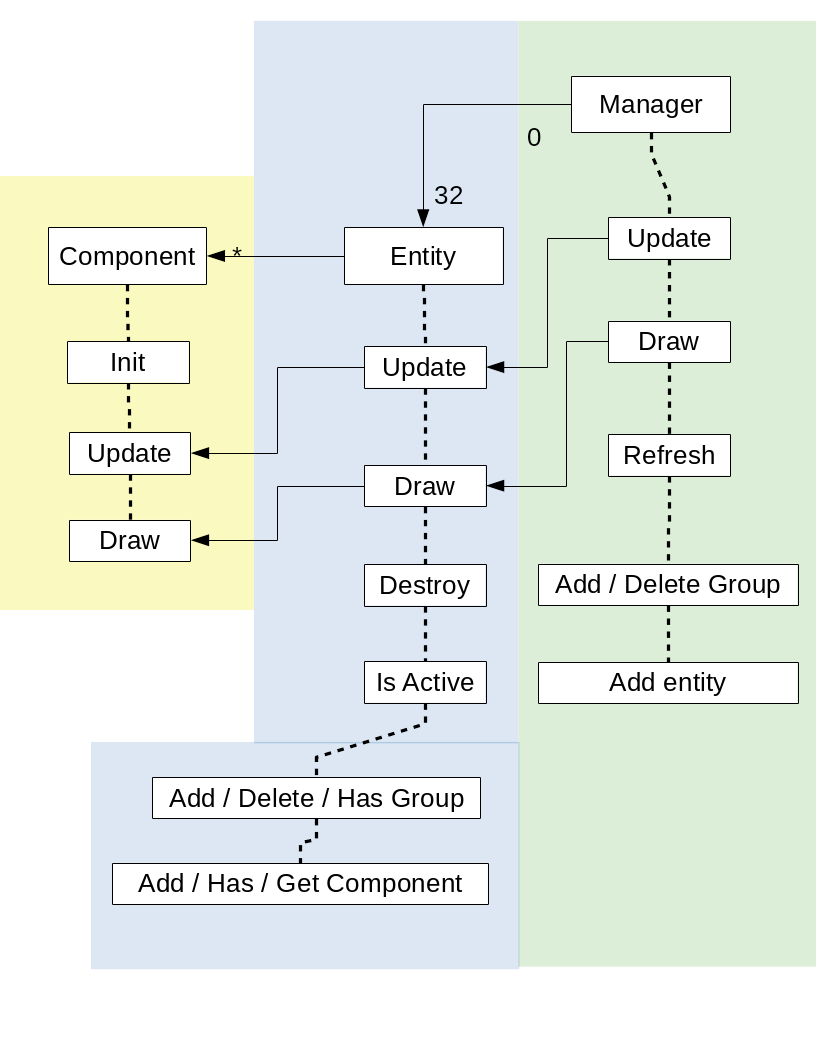
\includegraphics[scale=0.3]{Scheme}
  \caption{Entity-Component-System Verhältnisse}
  \label{fig:ECS}
\end{figure}

Man kann sich \textbf{Comopnents} als Container vorstellen. Sie besitzen keine
komplexe Logik. Jeder Typ einer \textit{Component} kann an ein \textit{Entity}
angebracht werden, um eine Art Eigenschaft bereitzustellen. Zum Beispiel macht
eine \textit{Collider-Komponente} eine \textit{Entity} zu einem starren Objekt. \\
Die \textbf{Entities} werden hauptsächlich verwendet, um einen eindeutige
Bezeichner anzubieten. Auf diese Weise wird die Umgebung auf die Existenz
einzelner, individueller \textit{Entities} aufmerksam. Eine \textbf{Entity}
wirkt als Root-Objekt, das eine Reihe von \textit{Components} bündelt. \\
Der \textbf{Manager (System)} wirkt als System-Teil des implementierten
Entwurfsmusters. Es besitzt keine \textit{Entity}, sondern greift auf sie zu, um
den Dateizyklus ihres \textit{Components} zu verwalten.

\section{Physik}
In diesem Projekt geht es um die Physik und deren Simulation in einer virtuellen
Umgebung. Die grundlegenden Gesetze, die implementiert werden, sind
Beschleunigung, Kollisionserkennung, Kollisionsauflösung und Partikel. Das
\textit{Transform Component} wurde zwecks die Simulation dieser Gesetze erstellt.

\begin{lstlisting}[language=C++]
  class TransformComponent : public Component
  {
    private:
    Vector2D position;
    Vector2D velocity;

    int speed  = 3;
    int width  = 32;
    int height = 32;
    int scale  = 1;

    float step;
    float acceleration;
    float friction = 0.2;
        ...
        ...
        ...
  };
\end{lstlisting}

Diese \textit{Components} enthält die meisten erforderlichen Eigenschaften für
ein Element, das in einem bestimmten Bereich definiert werden soll. Es werden
auch die Attribute festgelegt, die für die Bewegung des Gegenstands in diesem
Bereich erforderlich sind.
Die Bewegung erfolgt über die Begriffe Geschwindigkeit als skalare Größe,
Beschleunigung, Reibung und Geschwindigkeit als Vektorgröße. \\
\textbf{Geschwindigkeit als eine skalare Größe} kann als das Tempo betrachtet
werden, mit dem ein Objekt die Entfernung zurücklegt. Stellen Sie sich ein
Objekt mit hoher Geschwindigkeit vor. Gemäß der obigen Definition würde dies
bedeuten, dass das Objekt in kurzer Zeit eine relativ große Entfernung
zurücklegen würde. \\
\textbf{Die Geschwindigkeit als eine Vektorgröße} bezieht sich auf die Rate, mit
der ein Objekt seine Position ändert. \\
Der Hauptunterschied zwischen den beiden Begriffen ergibt sich aus der Tatsache,
dass Geschwindigkeit als skalare Größe die Richtung nicht verfolgt, während
Geschwindigkeit als Vektorgröße richtungsbewusst ist. \\
Man kann die \textbf{Beschleunigung} als Vektorgröße definieren, die die
Geschwindigkeit darstellt, mit der ein Objekt sein Tempo ändert. In anderen
Worten, ein Objekt beschleunigt sich, wenn es seine Geschwindigkeit ändert. \\
Der Begriff Reibung ist definiert als jede Kraft, die einer Relativbewegung
widersteht. \\
Die Beschleunigung wird als Eigenschaft des \textit{Transform Components}
eingeführt.
Mit jedem Frame wird sein Wert um einen bestimmten Schritt erhöht.

\begin{lstlisting}[language=C++]
    this->acceleration += this->step;

    if( this->acceleration > 7 )
        this->acceleration = 7;

    if( this->acceleration < 0 )
    {
        this->acceleration = 0;
        velocity.zero();
    }
\end{lstlisting}

Das implementierte Prinzip verwendet die Obergrenze für die Beschleunigung, um
sie realistischer aussehen. \\
Das einzige bewegliche Objekt ist der Avatar des Spielers. Sein Schritt ist mit
seiner Schaffung festgelegt.

\begin{lstlisting}[language=C++]
    player.addComponent< TransformComponent >( 2 );
    player.getComponent< TransformComponent >().setStep( 0.15 );
    player.addComponent< SpriteComponent >( "player", true );
    player.addComponent< KeyboardConstroller >( );
    player.addComponent< ColliderComponent >( "player" );
    player.addGroup( groupPlayer );
\end{lstlisting}

Die tatsächliche Bewegung der Hauptfigur wird vom Benutzer gesteuert. Durch
Drücken einer der Tasten --- ``w'', ``s'', ``a'' oder ``d'' wird die Trägheit des
Avatars verletzt. Die Definition dieses Inertionsprinzips ist definiert als die
Tendenz eines Objekts, Änderungen seiner Geschwindigkeit als Vektorgröße zu
widerstehen. Mit anderen Worten, wenn der Spieler die Bewegungstasten drückt,
wird die Trägheit des Avatars verletzt und seine Geschwindigkeit als Vektorgröße
geändert, wodurch sich seine Position ändert. \\

\begin{lstlisting}[language=C++]
    case SDLK_w:
        transform->getVelocity().setY( -1 );
        sprite->play( "walkUp" );
	break;
    case SDLK_a:
	transform->getVelocity().setX( -1 );
	sprite->play( "walkSideway" );
	sprite->spriteFlip = SDL_FLIP_HORIZONTAL;
	break;
    case SDLK_d:
	transform->getVelocity().setX( 1 );
	sprite->play( "walkSideway" );
	break;
    case SDLK_s:
	transform->getVelocity().setY( 1 );
	sprite->play( "walkDown" );
	break;
\end{lstlisting}

Zur leichteren Durchführung sind die Reibungsverläufe konstant. In Kombination
mit der eingestellten Geschwindigkeit als Vektorgröße werden die Geschwindigkeit
als Skalargröße und der Wert der Beschleunigung für das aktuelle Bild zur
aktuellen Koordinate des Avatars addiert. Auf diese Weise wird das Zeichen im
nächsten Frame an einer anderen Stelle angezeigt.

\begin{lstlisting}[language=C++]
    position.setX(
        tempX
        + velocity.getX()
        * this->speed
        * this->friction
        * this->acceleration
    );
    position.setY(
        tempY
        + velocity.getY()
        * this->speed
        * this->friction
        * this->acceleration
    );
\end{lstlisting}

Der Avatar des Spielers ist das einzige Objekt, das sich innerhalb der Welt frei
bewegt. Die restlichen Spielobjekte werden normalerweise aufgrund der
Kollisionsauflösung verschoben. Unter Spielobjekt fällt alles andere, was nicht
das Gelände, der Spieler oder die abgefeuerten Geschosse ist und in der Welt
angezeigt wird. Sie werden mit einer anderen Komponente --- Object Component
--- implementiert.

\begin{lstlisting}[language=C++]
class ObjectComponent : public Component
{
private:
    TransformComponent* transform;
    int durability = 1;
    bool isStatic = true;
    int mass = 1;
    ...
    ...
    ...
};
\end{lstlisting}

Ein Objekt in der virtuellen Umgebung befindet sich in Ruhe, bis es einen Impuls
erhält. Dieses Ereignis ist das Ergebnis einer Kollisionsauflösung. Wenn ein
solches Ereignis auftritt, erhält das Spielobjekt eine Beschleunigung und
verwendet seine Eigenschaftsmasse, um die Geschwindigkeit zu regulieren, mit der
diese Beschleunigung abnimmt.

\begin{lstlisting}[language=C++]
  if(transform->getAcceleration() > 0)
      transform->decAcceleration(transform->getStep() * mass);
\end{lstlisting}

\paragraph{}
Wenn es Objekte in Bewegung gibt, besteht auch die Möglichkeit, dass sie
kollidieren. Die Erkennung für dieses Ereignis erfolgt in jedem Frame am Ende
der Aktualisierungsphase. Um eine Kollision zwischen Objekten zu erkennen, wurde
das \textit{Collider Component} implementiert.

\begin{lstlisting}[language=C++]
  class ColliderComponent : public Component
  {
    private:
        std::string tag;
        SDL_Rect collider;
        TransformComponent* transform;
        ...
        ...
        ...
  };
\end{lstlisting}

Der Collider ist ein Rechteck um seine Entities mit zusätzlichen Eigenschaften
--- Tag und Transform Component. Jedes Entity, an der eine solche Komponente
angebracht ist, wird in die Kollisionserkennung einbezogen und gilt als starren
Körper. Das Tag des Colliders bestimmt seinen Typ. Auf diese Weise kann bei
einer Kollision zwischen zwei Entities leichter bestimmt werden, wie sie
behandelt werden sollen. Für die Position innerhalb der virtuellen Welt des
Colliders wird die Transform Component der Entity verwendet, an die der Collider
angehängt ist. Auf diese Weise ist sichergestellt, dass sich der Collider immer
um sein Objekt befindet. \\
Die Kollisionserkennung ist die einfachste Variante des Algorithmus ``Axis
Aligned Bounding Box''. Mit anderen Worten, wenn eine Lücke zwischen einer der
Seiten von zwei Kollidern gefunden wird, wird angenommen, dass sie kollidiert
sind.

\begin{figure}[h]
  \centering
  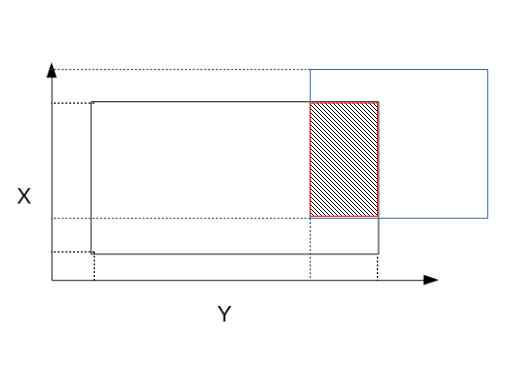
\includegraphics[scale=0.75]{AABB_Collision}
  \caption{Kollisionserkennung}
  \label{fig:Kollisionserkennung}
\end{figure}

Bei einer Kollision sollte die entsprechende Lösung durchgeführt werden. Zu
Beginn der Aktualisierungsphase wird die Position des Avatars des Spielers in
einer zeitlichen Variablen gespeichert.

\begin{lstlisting}[language=C++]
Vector2D playerPos = player.getComponent<TransformComponent>().getPosition();
\end{lstlisting}

Auf diese Weise würden die Lösungen des Spielers und eines kollidierenden
Spielobjekts die alte Position des Avatars zum Zurücksetzen verwenden und ein
Anstoßen in einem starren Körper simulieren. Aufgrund der unterschiedlichen
Arten von Kollisionsauflösungen erfolgt die Erkennung des Auftretens von
Kollisionen schrittweise. Die erste Kollisionsprüfung wird für den Spieler und
jeden anderen Kollider durchgeführt. Auf diese Weise kann in der erstellten
virtuellen Umgebung kein Objekt durchgelaufen werden.

\begin{lstlisting}[language=C++]
for( auto& coll : colliders )
{
    SDL_Rect tempColl = coll->getComponent<ColliderComponent>().getCollider();
    if(Collision::AABB(tempColl, playerColl))
    {
        player.getComponent<TransformComponent>().setPosition(playerPos);
    }
}
\end{lstlisting}

Die nächste Kollisionsprüfung betrifft die Projektile. Zuerst wird geprüft, ob
ein Projektil den Spieler getroffen hat. In der aktuellen Version ist es jedoch
redundant, da in der Spielumgebung außer dem Player nichts anderes vorhanden
ist, das Projektile abfeuert. Die Prüfung erfolgt in zwei Schritten, da es
unterschiedliche Arten der Kollisionsauflösung gibt. Die Lösung für ein
Projektil, das einen Spieler trifft, besteht darin, dass zuerst eine
Konsolenmeldung zu Debugging-Zwecken ausgedruckt wird und dann das Projektil zu
zerstören. Die Auflösung für ein Projektil, das auf ein Spielobjekt trifft, ist
unterschiedlich, da sich das Spielobjekt bewegen sollte, wenn es nicht statisch
ist, mit anderen Worten, das Spielobjekt funktioniert wie ein Teil des Geländes.
Die Spielobjekte haben eine Haltbarkeit, die mit jedem Treffer des Projektils
abnimmt. Die statischen Spielobjekte haben eine nahezu unendliche Haltbarkeit.
Aus diesem Grund erfolgt die Auflösung in verschiedenen Schritten. Die
beweglichen Objekte in der Spielszene werden als Kästchen dargestellt. Wenn das
Projektil auf eine Box trifft, wird der Schritt, mit dem sich das Projektil
bewegt, als Schritt auf die Box gesetzt. Die Beschleunigung und die
Geschwindigkeit des Projektils werden ebenfalls an die Box übergeben. Auf diese
Weise wird der Impuls simuliert, der an das Spielobjekt weitergegeben werden
soll, wenn etwas darauf trifft, in diesem Fall das Projektil. Nachdem der Impuls
verstrichen ist, verringert sich die Haltbarkeit des Objekts und das Projektil
wird zerstört.

\begin{lstlisting}[language=C++]
if( Collision::AABB(
    proj->getComponent<ColliderComponent>().getCollider(),
    gObj->getComponent<ColliderComponent>().getCollider()) &&
    !gObj->getComponent<ObjectComponent>().getIsStatic())
{
    printf( "An object was hit!\n" );
    proj->destroy();
    gObj->getComponent<TransformComponent>().setStep(
        proj->getComponent<TransformComponent>().getStep()
    );
    gObj->getComponent<TransformComponent>().setAcceleration(
        proj->getComponent<TransformComponent>().getAcceleration()
    );
    gObj->getComponent<TransformComponent>().setVelocity(
        proj->getComponent<TransformComponent >().getVelocity()
    );
    gObj->getComponent<ObjectComponent>().decDurability(1);
}
\end{lstlisting}

Die dritte unterschiedliche Projektilkollisionsauflösung wird durchgeführt, um
ein statisches Spielobjekt mit einem Projektil zu treffen. In diesem Fall wird
eine Meldung gedruckt, und das Projektil wird zerstört, und die Lebensdauer des
Objekts nimmt ab.

\begin{lstlisting}[language=C++]
  if( Collision::AABB(
    proj->getComponent<ColliderComponent>().getCollider(),
    gObj->getComponent<ColliderComponent>().getCollider() )
    && gObj->getComponent<ObjectComponent>().getIsStatic() )
    {
	printf("An static game object was hit.\n");
	proj->destroy();
	gObj->getComponent<ObjectComponent>().decDurability(1);
    }
\end{lstlisting}

Wenn der Avatar des Spielers gegen ein bewegliches Spielobjekt stößt, wird dies
ähnlich wie beim Auftreffen eines Projektils auf eine Schachtel aufgelöst. Der
Schritt, die Beschleunigung und die Geschwindigkeit des Spielers werden an die
Box übergeben, während der Avatar vor der Kollision an seine Position
zurückgebracht wird. Die Beschleunigung des Spielers wird auf Null gesetzt.

\begin{lstlisting}[language=C++]
player.getComponent<TransformComponent>().setPosition(playerPos);
gObj->getComponent<TransformComponent>().setStep(
    player.getComponent<TransformComponent>().getStep()
);
gObj->getComponent<TransformComponent>().setAcceleration(
    player.getComponent<TransformComponent>().getAcceleration()
);
gObj->getComponent<TransformComponent>().setVelocity(
    player.getComponent<TransformComponent>().getVelocity()
);
player.getComponent<TransformComponent>().setAcceleration(0.0f);
\end{lstlisting}

Wenn der Spieler mit einem statischen Spielobjekt kollidiert, stößt er den
Charakter gegen eine Wand. In der aktuellen Version der virtuellen Welt sind
Wände die Endteile der Karte. Wenn ein solches Ereignis eintritt, wird die
Position des Avatars des Spielers zurückgesetzt und seine Beschleunigung auf 0
gesetzt.

\begin{lstlisting}[language=C++]
player.getComponent<TransformComponent>().setPosition(playerPos);
player.getComponent<TransformComponent>().setAcceleration(0);
\end{lstlisting}

Die komplizierteste Lösung ist die Kollision zweier Spielobjekte. Dies kann
ausgelöst werden, wenn der Benutzer oder ein Projektil gegen ein Spielobjekt
stößt und sich dieses Spielobjekt in unmittelbarer Nähe eines anderen befindet
und auf dieses trifft. Die Auflösung verwendet die Position eines Spielobjekts,
um sich daran zu erinnern, wo sich das Objekt befand, bevor es gegen ein anderes
Spielobjekt stieß. Wenn eine Kollision auftritt, überträgt das Objekt, das in
das umgebende Objekt geschoben wurde, seine Schritte, Beschleunigungen und
Geschwindigkeiten auf das andere Spielobjekt. Danach wird seine Beschleunigung
auf 0 gesetzt.

\begin{lstlisting}[language=C++]
nextGObj->getComponent<TransformComponent>().setStep(
    gObj->getComponent<TransformComponent>().getStep(
));
nextGObj->getComponent<TransformComponent(
    gObj->getComponent<TransformComponent>().getAcceleration()
);
nextGObj->getComponent<TransformComponent>().setVelocity(
  gObj->getComponent<TransformComponent>().getVelocity()
);
\end{lstlisting}

Ein weiterer Bestandteil der Implementierung der Physik ist die Implementierung
des Projektils als Komponente. Ein Projektil wird durch seine aktuelle Position
in der virtuellen Welt, die maximale Reichweite, die es zurücklegen sollte,
bevor es zerstört wird, die aktuelle zurückgelegte Distanz und seine
Geschwindigkeit definiert.

\begin{lstlisting}[language=C++]
class ProjectileComponent : public Component
{
private:
    TransformComponent* transform;
    int range    = 0;
    int speed    = 0;
    int distance = 0;
    Vector2D velocity;
    ...
    ...
    ...
}
\end{lstlisting}

Das Projektil wird zerstört, wenn es seinen festgelegten Maximalbereich
überschritten hat oder um die Leistung zu verbessern, wenn sich das Projektil
nicht mehr in der Sichtweite des Benutzers befindet. In beiden Fällen wird eine
entsprechende Meldung angezeigt.

\begin{lstlisting}[language=C++]
if( distance > range )
{
    printf("Out of range\n");
    entity->destroy();
}
else if(transform->getXPos() > Game::camera.x + Game::camera.w ||
    transform->getXPos() < Game::camera.x ||
    transform->getYPos() > Game::camera.y + Game::camera.h ||
    transform->getYPos() < Game::camera.y)
{
    printf("Out of bounds\n");
    entity->destroy();
}
\end{lstlisting}

\section{Fazit}
Ziel des Projekts war es, die gängigsten physikalischen Gesetze in eine
virtuelle Umgebung umzusetzen. Als Ergebnis wurde ein einfaches Spiel erstellt,
in dem die Implementierung demonstriert wurde. Der Benutzer interagiert mit der
virtuellen Welt über eine Avatar-Figur, die er steuert. Die Hauptfigur des
Spiels bewegt sich, wie es die implementierte Physik demonstriert ---
Beschleunigung, Kollisionserkennung und -auflösung, einfache Partikel. \\
Um die Einführung der Physik in das Spiel und die Pflege der Daten zu
vereinfachen, wurde eine einfache Konstruktion ähnlich dem Designmuster
``Entity-Component-System'' entwickelt. \\
Die Physik ist so einfach wie möglich implementiert. Aufgrund dieses Spiels
bleiben Objekte mit geringerer Masse, die beschleunigt und gegen ein Objekt mit
größerer Masse gestoßen werden, ineinander stecken. Die implementierte
Kollisionserkennung würde auch abnehmen, wenn eine genauere Erkennung
erforderlich ist. \\
Das Projekt ist der Einstieg in die Computerphysik. Von diesem Punkt an könnte
man sich auf das Polieren des implementierten Algorithmus konzentrieren, so dass
die Implementierungen in einem breiteren Bereich von Fällen anwendbar sind. Es
ist auch eine gültige Entwicklung, einen Teil des Gesetzes über die optische
Physik umzusetzen.

\end{document}
